\documentclass[pdftex,12pt]{article}
\usepackage{fullpage}
\usepackage{graphicx}
\usepackage{natbib}
\usepackage{amsmath}

\title{Storm Surges}

\date{\today}

\begin{document}
\maketitle

\begin{abstract}
Abstract to be completed
\end{abstract}

\section{Introduction}\label{sec:intro}
\citep{masson2004modelling} %testing a citation
%To be included: NEMO overview, tides, rivers, bathymetry, atmospheric forcing, vertical/lateral mixing, boundary conditions, grid. 

\section{Model Configuration}\label{sec:config}
%A section about how we configured the model for SoG 
\subsection{Model domain}
The modelled domain extends from the Strait of Juan de Fuca to Puget Sound to Johnstone Strait as shown in Figure \ref{fig:domain}. Bathymetry from the Cascadia physiography dataset \cite{?} was smoothed to limit the difference in depth across grid cells. For model stability, additional smoothing at the Strait of Juan de Fuca western boundary was performed to achieve constant depth across the first ten grid cells. 


\begin{figure}[h]
\centering
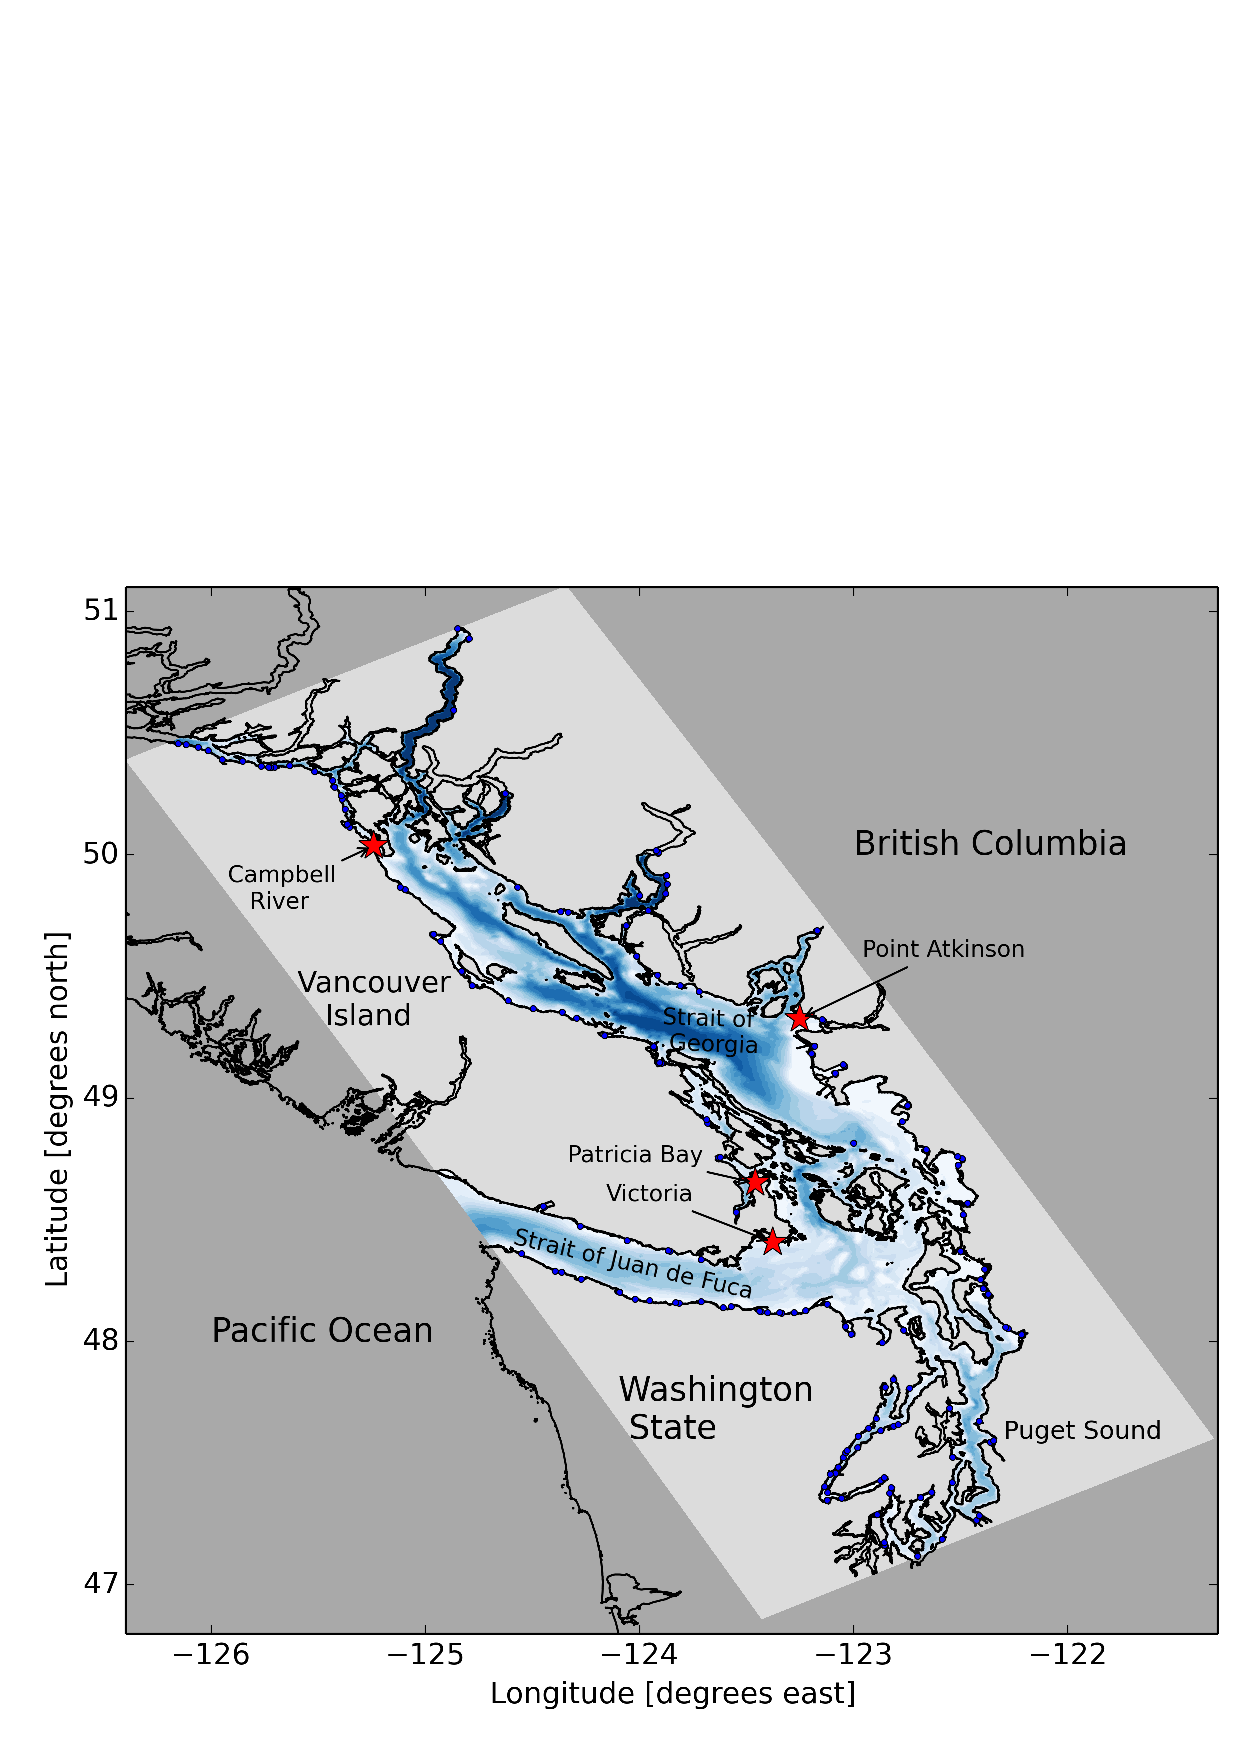
\includegraphics[scale=0.5]{Figures/bathy.png}
\caption{Model domain including bathymetry, rivers (*), and storm surge locations (o) of interest.}\label{fig:domain}
\end{figure}

\subsection{Boundary conditions}
%lateral and bottom friction, open boundaries, eta surface

\subsubsection{Tidal forcing} 
The model was forced by tidal elevations and currents at the Juan de Fuca and Johnstone Strait boundaries. Tidal heights and currents at grid points along the Juan de Fuca boundary were extracted from Webtide, an online web prediction model for the northeast Pacific Ocean, which is based on \citep{foreman2000webtide}. The Johnstone Strait boundary was forced with...? (e.g. we might use tidal harmonics measured and calculated by \citep{thomson1980johnstone})

\subsubsection{Temperature and salinity}
Temperature and salinity at the Juan de Fuca boundary were taken from a weekly climatology which was created from results from a model covering the Salish Sea and the west coast of Vancouver Island \citep{massonfine2012}.  Their results, originally on s-levels were interpolated onto z-levels and then onto the NEMO horizontal grid.  To prepare the climatology all years (1995-2008) were averaged and results, approximately every 15 days, were interpolated to a weekly climatology.

\subsubsection{Sea Surface Height}
Sea surface height at the mouth of Juan de Fuca was set using values from the Tofino tide guage.  A monthly climatology was produced using daily averages from 2000-2010, binning them by month, averaging and setting the yearly mean to zero.  For the storm surge simulations, hourly variations in sea surface height were used.  These values are the Tofino tide guage values, de-tided and with the zero reset as for the climatology.

\subsubsection{Open Boundary Conditions}

The model relaxed to the forced temperature and salinity over the 10 grid points (about 5km) closest to the open boundaries, using the NEMO FRS scheme \cite.  The tidal forcing and sea surface height was used in the barotropic velocity forcing which used the NEMO Flather scheme \cite  The baroclinic velocities at the boundary were set to be equal to the values inside the boundary (zero-gradient boundary conditions).  This scheme is not part of core NEMO.  Zero gradient conditions were chose because the baroclinic velocity at the mouth of Juan de Fuca is primarily estuarine and thus set by density variations between inside and outside the domain.

\subsection{River forcing} %Kate
River input provides a significant volume of freshwater to the Salish Sea and can influence stratification, circulation and primary productivity. However, most rivers in the domain are not gauged so parameterisations were required to represent river flow. \citep{morrison2011rivers} provides a method for estimating freshwater runoff in the Salish Sea region based on precipitation. Monthly runoff volumes for each watershed for each year from 1970 to 2012 were acquired from \citep{morrison2011rivers}, as well as monthly averages. 

Freshwater runoff from each watershed was divided between the rivers in that watershed. The area drained by each river was estimated from Toporama maps by the Atlas of Canada and watershed maps available on the Washington State government website. The watersheds included in our model were Fraser (which represents approximately 44\% of the freshwater input into our domain), Skagit (12\%), East Vancouver Island (North and South) (12\%), Howe (7\%), Bute (7\%), Puget (6\%), Juan de Fuca (5\%), Jervis (4\%) and Toba (3\%). 

The monthly flow from each river was input as a point source in the three grid points closest to the surface at the model point closest to the mouth of each river. Incoming water was assumed to be fresh, with a temperature of ?? degrees C. A total of 150 rivers were parameterised by this method. 

%we could show the location of all the rivers on the overall location map, or on a picture of our domain, since the rivers are on the edges of the domain so they won't block any bathymetry information

\subsection{Atmospheric forcing}

\subsection{Initial conditions}
Initial conditions for temperature and salinity were taken from a CTD cast in the middle Strait of Georgia taken in Sept 2002 \citep{pawlowiczetal2007}.  Conditions were initially uniform horizontally.  Velocity was initialized at zero.

\subsection{Spin-up}
The model was spun up for a 15.5 months from the initial conditions above, starting Sep 16, 2002, using atmospheric forcing from 2002-2003, climatological temperature and salinity and sea surface height at the boundaries, with tides and climatological river output.  All storm surge runs were started.....

\section{Model Evaluation}\label{sec:model}

\subsection{Tidal evaluation}
The model was initially evaluated qualitatively by comparing patterns of tidal amplitude and phase to results from \citep{foreman1995tidal}. For example, the amphidromic dome around Victoria was produced in the $M_2$ results, as well as the monotonic decrease in $M_2$ amplitude moving northwards along the Strait of Georgia. Initially, the Johnstone Strait boundary was closed, but modelled $M_2$ amplitudes were too small compared to measured amplitudes... TBC

%perhaps a nice contour map of M2 and K1 amps and phases goes here?

Once our model was reproducing observed tidal patterns, model results were quantitatively evaluated by comparing modelled harmonic constituents to measured harmonic constituents at tidal measuring stations throughout the domain. Comparisons were made using the complex difference (D), defined by \citep{foreman1995tidal} as:

\begin{equation}
D = [(A_0 \cos g_0 - A_m \cos g_m)^2 + (A_0 \sin g_0 - A_m \sin g_m)^2]^{1/2}
\end{equation}
where $A_0$, $A_m$, $g_0$ and $g_m$ are observed and modelled amplitudes and phases.

%perhaps a table of complex differences at tidal stations similar to Table 1 of Foreman et al (1995)  (such as the one produced by tidetools.calc_diffs_meas_mod) here?
%(would be cool to include the complex differences calculated at the VENUS nodes too)

Complex differences were less than ??cm at all stations in our domain, which was assumed to be acceptable for our purposes. 
%if it's favourable, we could compare our complex differences to Foreman et al (1995), who got an average of D=3cm for M2 and D=2.5cm for K1

\section{Storm Surge Hindcasts}\label{sec:storm}

\section{Conclusions}\label{sec:conclusions}


\bibliographystyle{plain}
\bibliography{ref}

\end{document}

